% Templates
\lstset{inputpath=source/1-introduction/}

\subsection{Template C++}
\lstinputlisting[language=c++]{template.cpp}

\subsection{Template Java}
\lstinputlisting[language=java]{template.java}

\subsection{Template Python 3.6}
\lstinputlisting[language=Python]{template.py}

\subsection{Bit Operations}
\lstinputlisting[language=c++]{bitmanip.cpp}

% ====================================================================================================
% Data Structures
\section{Data Structures}
\lstset{inputpath=source/2-data-structures/}

\subsection{Efficient Segment Tree}
\lstinputlisting[language=c++]{SegmentTree-efficient.cpp}

\subsection{Persistent Segment Tree}
\lstinputlisting[language=c++]{SegmentTree-persistent.cpp}

\subsection{Binary Indexed (Fenwick) Tree}
\lstinputlisting[language=c++]{BinaryIndexedTree.cpp}
\begin{verbatim}
Range [l..r] Update
upd(BITree1, l, val);    upd(BITree2, l, val*(l-1));
upd(BITree1, r+1, -val); upd(BITree2, r+1, -val*r);
Range [1..k] Query
que(BITTree1, k)* k - que(BITTree2, k);
\end{verbatim}

\subsection{AVL Tree}
\textbf{Let}
\begin{verbatim}
z as first unbalanced node
y as larger height child of z
x as larger height child of y
\end{verbatim}

\textbf{Case}
\begin{verbatim}
z  -->L  y  -->L  x  (LL Case): rotateRight(z)
z  -->L  y  -->R  x  (LR Case): rotateLeft(y), rotateRight(z)
z  -->R  y  -->L  x  (RL Case): rotateRight(y), rotateLeft(z)
z  -->R  y  -->R  x  (RR Case): rotateLeft(z)
\end{verbatim}

\textbf{Rotation}
\begin{verbatim}
||         y                              x          ||
||        / \       Right Rotation       /  \        ||
||       x   T3     - - - - - - - >     T1   y       ||
||      / \         < - - - - - - -         / \      ||
||     T1  T2       Left Rotation         T2  T3     ||
\end{verbatim}

\subsection{Link Cut Tree}
\lstinputlisting[language=c++]{LinkCut-Tree.cpp}

\subsection{Tries}
\lstinputlisting[language=c++]{Tries.cpp}

\subsection{Mo Algorithm}
\lstinputlisting[language=c++]{Mo-Algorithm.cpp}

\subsection{Misof Tree}
\lstinputlisting[language=c++]{Misof-Tree.cpp}

\subsection{Heavy-Light Decomposition}
\lstinputlisting[language=c++]{HeavyLightDecomposition.cpp}

% ====================================================================================================
% Data Structures
\section{Dynamic Programming}
\lstset{inputpath=source/3-dynamic-programming/}

\subsection{LIS (Longest Increasing Subsequence)}
\lstinputlisting[language=c++]{LongestIncreasingSubsequence.cpp}

\subsection{Cyclic LCS (Longest Common Subsequence)}
\lstinputlisting[language=c++]{LongestCommonSubsequence-cyclic.cpp}

\subsection{Longest Common Increasing Subsequence}
\lstinputlisting[language=c++]{LongestCommonIncreasingSubsequence.cpp}

\subsection{DP Buka String dan Lipat String}
\lstinputlisting[language=c++]{../9-etc/DP-Buka-String-Lipat-String.cpp}

\subsection{Matrix Chain Multiplication}
\lstinputlisting[language=c++]{MatrixChainMultiplication.cpp}

\subsection{Min Cut Polygon Triagulation}
\lstinputlisting[language=c++]{MinCutPolygonTriagulation.cpp}

\subsection{Kadane}
\lstinputlisting[language=c++]{Kadane.cpp}

\subsection{DP SOS}
\lstinputlisting[language=c++]{DP-SOS.cpp}

\subsection{DP Convex Hull}
\lstinputlisting[language=c++]{DP-ConvexHull.cpp}

\subsection{DP Divide and Conquer}
\lstinputlisting[language=c++]{DP-DivideAndConquer.cpp}

\subsection{DP Knuth Yao}
\lstinputlisting[language=c++]{DP-KnuthYao.cpp}

% ====================================================================================================
% Graphs
\section{Graphs}
\lstset{inputpath=source/4-graphs/}

\subsection{Link Cut Tree}
\lstinputlisting[language=c++]{TopologicalSort-recursive.cpp}
Kahn's Algorithm
\lstinputlisting[language=c++]{TopologicalSort-KahnAlgorithm.cpp}

\subsection{k-th Shortest Path}
\lstinputlisting[language=c++]{ShortestPath-kth.cpp}

\subsection{Manhattan Spanning Tree}
\lstinputlisting[language=c++]{SpanningTree-manhattan.cpp}

\subsection{Directed MST}
\lstinputlisting[language=c++]{SpanningTree-directed.cpp}

\subsection{Bellman Ford (Negative Cycle Detection)}
\lstinputlisting[language=c++]{BellmanFord.cpp}

\subsection{Dinic Algorithm}
\lstinputlisting[language=c++]{Flow-DinicAlgorithm.cpp}

\subsection{LowestCommonAncestor (SegTree)}
\lstinputlisting[language=c++]{LowestCommonAncestor-SegTree.cpp}
\begin{verbatim}
Let LCA(r,u,v) be the LCA of u and v with respect to root r. To
compute LCA(r,u,v), we can compute, for any fixed ro (let ro = 1),
LCA(ro,r,u);    // LCA(1,r,u);
LCA(ro,r,v);    // LCA(1,r,v);
LCA(ro,u,v);    // LCA(1,u,v);
and take the "odd man out". Otherwise, take any one.
\end{verbatim}


\subsection{Min Cost Max Flow}
\lstinputlisting[language=c++]{Flow-MinCostMaxFlow.cpp}

\subsection{Min Cost Max Flow (Multiple Edges)}
\lstinputlisting[language=c++]{Flow-MinCostMaxFlow-MultiEdges.cpp}

\subsection{Max Flow (Adj List)}
\lstinputlisting[language=c++]{Flow-MaxFlow-adjList.cpp}

\subsection{Min Cut (Stoer Wagner)}
\lstinputlisting[language=c++]{MinCut-StoerWagner.cpp}

\subsection{Eulerian Tour Checking}
\lstinputlisting[language=c++]{EulerianTour-checking.cpp}

\subsection{Max Bipartite Matching}
\lstinputlisting[language=c++]{MaxBipartiteMatching-alternatingPath.cpp}

\subsection{Minimum Vertex Cover}
\lstinputlisting[language=c++]{MinimumVertexCover.cpp}

\subsection{Articulation Point and Bridge}
\lstinputlisting[language=c++]{ArticulationPointBridge.cpp}

\subsection{SCC - Tarjan Algorithm}
\lstinputlisting[language=c++]{StronglyConnectedComponents-Tarjan.cpp}

\subsection{SCC - Kosaraju Algorithm}
\lstinputlisting[language=c++]{StronglyConnectedComponents-Kosaraju.cpp}

\subsection{Hopcroft Karp}
\lstinputlisting[language=c++]{HopcroftKarp.cpp}

\subsection{Euler Path + Euler Tour}
\lstinputlisting[language=c++]{EulerianTour-path.cpp}

\subsection{Edmonds Blossom}
\lstinputlisting[language=c++]{EdmondsBlossom.cpp}

\subsection{Aho Corasick}
\lstinputlisting[language=c++]{../6-string-processing/AhoCorasick.cpp}

\subsection{Maximum Clique}
\lstinputlisting[language=c++]{MaximumClique.cpp}

\subsection{DSU on Tree}
\lstinputlisting[language=c++]{../2-data-structures/DisjointSetsUnion-onTree.cpp}

\subsection{Recover Min-Vertex Cover from Maximum Matching}
\begin{verbatim}
Suppose you have left and right parts in bipartite graph and you found the
maximum matching M. Let's define orientation of edges. Those edges that belong
to M will go from right to left, all other edges will go from left to right.
Now run DFS starting at all left vertices that are not incident to edges in M.
Some vertices of the graph will become visited during this DFS and some
not-visited. To get minimum vertex cover you take all visited right vertices of
M, and all not-visited left vertices of M.
\end{verbatim}


% ====================================================================================================
% String Processing
\section{String Processing}
\lstset{inputpath=source/6-string-processing/}

\subsection{KMP Algorithm}
\lstinputlisting[language=c++]{KMP.cpp}

\subsection{Suffix Array}
\lstinputlisting[language=c++]{SuffixArray.cpp}
\lstinputlisting[language=c++]{SuffixArray_hantansu98.cpp}

\subsection{Enhanced Suffix Array}
\lstinputlisting[language=c++]{SuffixArray-enhanced.cpp}

\subsection{Edit Distance}
\lstinputlisting[language=c++]{EditDistance.cpp}

\subsection{kth Permutation}
\lstinputlisting[language=c++]{Permutation-kth.cpp}

\subsection{Manacher's Algorithm (Longest Palindromic Substring)}
\lstinputlisting[language=c++]{ManachersAlgorithm.cpp}

% ====================================================================================================
% Etc
\section{ETC}
\lstset{inputpath=source/9-etc/}

\subsection{Soal TIMO 2010}
\lstinputlisting[language=c++]{SoalTimo2010.cpp}

\subsection{Meet in the Middle}
\lstinputlisting[language=c++]{MeetInTheMiddle.cpp}

\subsection{Huffman Code}
\lstinputlisting[language=c++]{HuffmanCode.cpp}

\subsection{Hungarian Algorithm}
\lstinputlisting[language=c++]{HungarianAlgorithm.cpp}

\subsection{Stable Marriage}
\lstinputlisting[language=c++]{StableMarriage.cpp}

\subsection{CSOD}
\lstinputlisting[language=c++]{CSOD.cpp}

\subsection{RDN (goto 0001/01/01)}
\lstinputlisting[language=c++]{RDN.cpp}

% ====================================================================================================
% Mathematics
\section{Mathematics}
\lstset{inputpath=source/5-maths/}

\subsection{Big Integer}
\lstinputlisting[language=c++]{BigInteger.cpp}

\subsection{Fast Fourier Transform + NTT}
\lstinputlisting[language=c++]{FFT+NTT.cpp}

\subsection{Gauss Elimination}
\lstinputlisting[language=c++]{GaussElimination.cpp}

\subsection{Number Theory}
\textbf{Bertrand's Ballot Theorem} \\
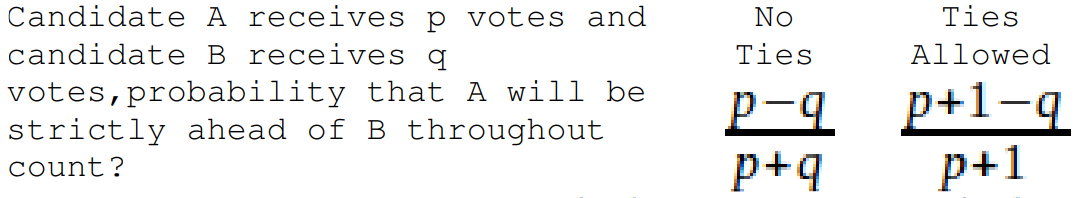
\includegraphics[width=\linewidth]{source/5-maths/Temporary/bertrandBallot.png}

\textbf{Gambler's Ruin Theorem} \\
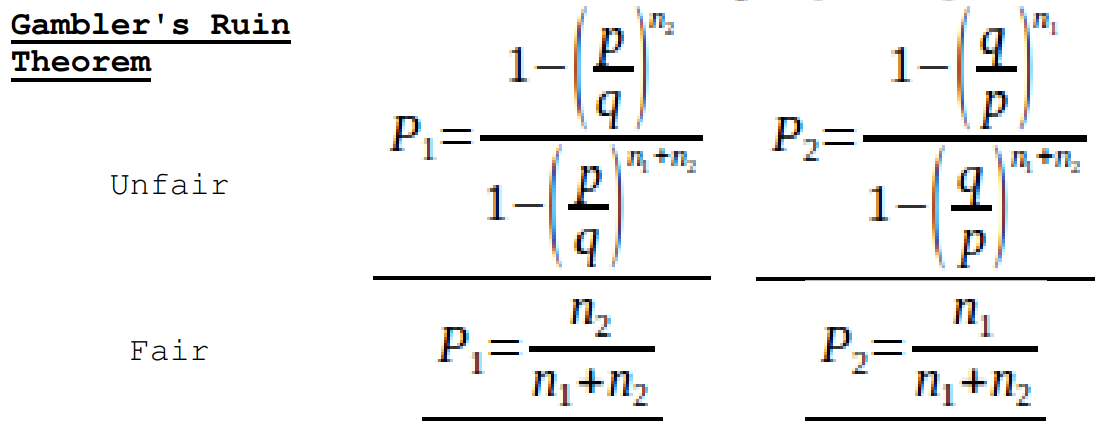
\includegraphics[width=\linewidth]{source/5-maths/Temporary/gamblersRuin.png}

\textbf{Pick Theorem} \\
Let A : the area of a simply closed lattice polygon; B : the number of lattice points on the Polygon edges; I : the number of points in the interior of the polygon. Then \textbf{A = I+(1/2)B-1}

\textbf{Forbenius Number} \\
If GCD is 1 then required largest amount is (X*Y)-(X+Y) and total count is (X-1)*(Y-1)/2

\textbf{Erdos Gallai Theorem} \\
A sequence of non-negative integers $ d_1 \leq \dotsc \leq d_n $, can be represented as the degree sequence of a finite simple graph on n vertices if and only if $ d_1 + \dotsc + d_n $ is even and $ \sum_{i=1}^{i=k} d_i \leq k (k-1) + \sum_{i=k+1}^{i=n} min(d_i,k) $, holds every $ 1 \leq k \leq n $.

\textbf{Derangement}
\begin{lstlisting}[language=c++]
ll der[15];   der[0] = 1;   der[1] = 0;
REP(i,2,10) der[i] = ((ll)i-1)*(der[i-1]+der[i-2]);
\end{lstlisting}

\textbf{Bell Number} \\
The number of ways a set of n elements can be partitioned into nonempty subsets
\begin{lstlisting}[language=c++]
ll bell[25+5][25+5];   bell[0][0] = 1;
REP(i,1,maks){
	bell[i][0] = bell[i-1][i-1];
	REP(j,1,i)bell[i][j]=bell[i-1][j-1]+bell[i][j-1];
} // Example : n=10 ==> bell[10][0]
\end{lstlisting}

\textbf{Stirling Number 2nd Kind} \\
The number of ways a set of n elements into k subsets) \\
Recurrence : S(n,k) = k*S(n-1,k) + S(n-1,k-1)
\begin{lstlisting}[language=c++]
int stir[n+1][k+1];
for (int i=0; i<=n; i++) stir[i][0] = 0;
for (int i=0; i<=k; i++) stir[0][k] = 0;
REP(i,1,n) REP(j,1,i){
	if (j == 1 || i == j) stir[i][j] = 1;
	else stir[i][j] = j*stir[i-1][j] + stir[i-1][j-1];
} // Example : n=3,k=1 : stir[3][1]
\end{lstlisting}

\textbf{Carmichael Number} \\
Composite numbers n such that a\^(n-1) == 1 (mod n) for every a coprime to n.
\begin{lstlisting}[language=c++]
// 561, 1105, 1729, 2465, 2821, 6601, 8911, 10585
// 15841, 29341, 41041, 46657, 52633, 62745, 63973
// 75361, 101101, 115921, 126217, 162401, 172081
// 188461, 252601, 278545, 294409, 314821, 334153
// 340561, 399001, 410041, 449065, 488881, 512461
\end{lstlisting}

\textbf{Vandermonde Convolution} \\
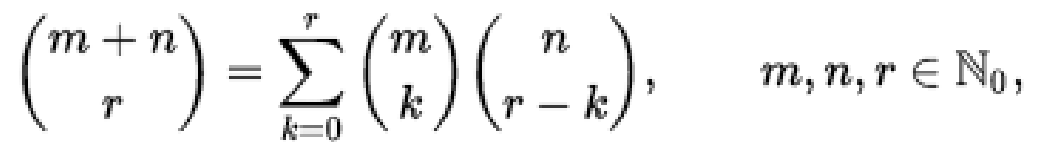
\includegraphics[width=\linewidth]{source/5-maths/Temporary/vandermonde.png}

\textbf{Q-Vandermonde Convolution} \\
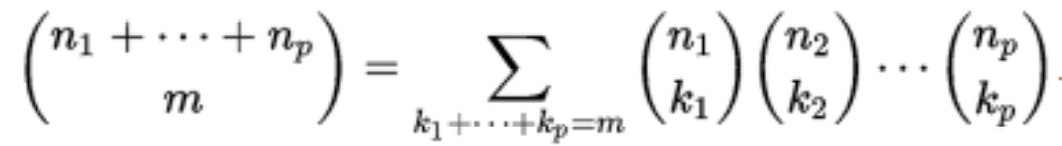
\includegraphics[width=\linewidth]{source/5-maths/Temporary/qVandermonde1.png}
\begin{multicols}{2}
	int m,n \\
	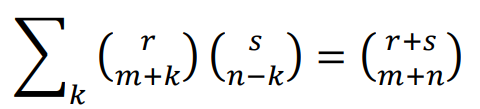
\includegraphics[width=\linewidth]{source/5-maths/Temporary/qVandermonde2.png} \\
	int $l \geq 0$, int m,n \\
	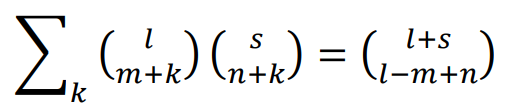
\includegraphics[width=\linewidth]{source/5-maths/Temporary/qVandermonde3.png}
\end{multicols}
int $l \geq 0$, int m,n \\
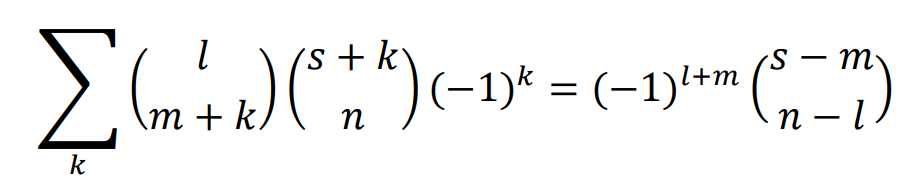
\includegraphics[width=\linewidth]{source/5-maths/Temporary/qVandermonde4.png} \\
int l,m, $m \geq 0$ \\
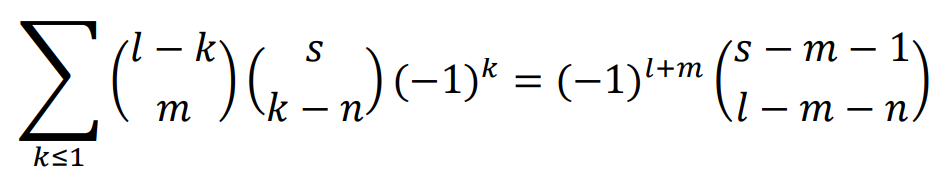
\includegraphics[width=\linewidth]{source/5-maths/Temporary/qVandermonde5.png} \\
int $l,m \geq 0$, int $n \geq q \geq 0$ \\
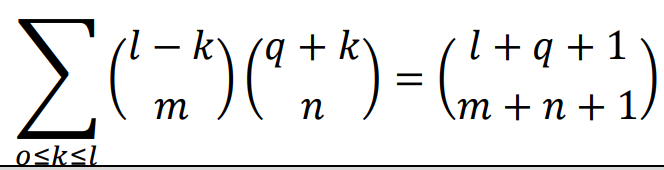
\includegraphics[width=\linewidth]{source/5-maths/Temporary/qVandermonde6.png}


\subsection{Necklace and Bracelets Combinatorics}
\begin{multicols}{2}
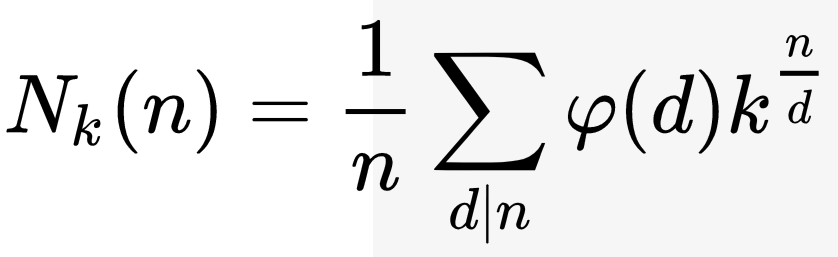
\includegraphics[width=0.8\linewidth]{source/5-maths/Temporary/necklace.png} \\
Aperiodic Necklace: change $\varphi$ to $\mu$ Mobius \\
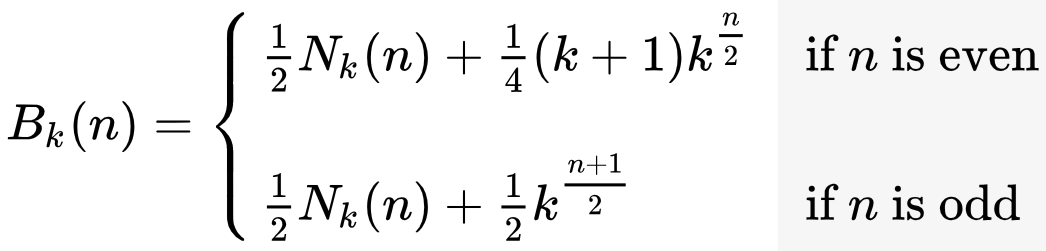
\includegraphics[width=\linewidth]{source/5-maths/Temporary/bracelets.png}
\end{multicols}

\subsection{Mathematics Sequence Formula}
\begin{large}
  \textbf{Faulhaber} O($p^2$) \\
  ${\displaystyle \sum _{k=1}^{n}k^{p}={1 \over p+1}\sum _{j=0}^{p}(-1)^{j}{p+1 \choose j}B_{j}n^{p+1-j}}$
  \hfill
  ${\displaystyle B_{n}={\begin{cases}{1}&{\text{: }}n=0\\{\displaystyle -\sum _{k=0}^{n-1}{n \choose k}{\frac {B_{k}}{n-k+1}}}&{\text{: }}n>0\end{cases}}}$
\end{large}


\subsection{Prime Number List}
\begin{verbatim}
10^ 1   7             10^11   99999999977
10^ 2   97            10^12   999999999989
10^ 3   997           10^13   9999999999971
10^ 4   9973          10^14   99999999999973
10^ 5   99991         10^15   999999999999989
10^ 6   999983        10^16   9999999999999937
10^ 7   9999991       10^17   99999999999999997
10^ 8   99999989      10^18   999999999999999989
10^ 9   999999937     10^19   9999999999999999961
10^10   9999999967
Below (2^31)-1: 2147483629 (is 8th Mersenne Prime)
Below (2^32)-1: 4294967291
Below (2^63)-1: 9223372036854775783
Below (2^64)-1: 18446744073709551557
\end{verbatim}

\subsection{Catalan and Super Catalan}
\lstinputlisting[language=c++]{Sequence-catalan.cpp}

\subsection{Digit Counting Factorial}
\lstinputlisting[language=c++]{Factorial-digitCounting.cpp}

\subsection{INT to ROMAN}
\lstinputlisting[language=c++]{Convert-intToRoman.cpp}

\subsection{Linear Diophantine}
\lstinputlisting[language=c++]{LinearDiophantine.cpp}

\subsection{Chinese Remainder Theorem}
\lstinputlisting[language=c++]{ChineseRemainderTheorem.cpp}
\lstinputlisting[language=c++]{ChineseRemainderTheorem_whyzker.cpp}

\subsection{Euler Totient (Phi) Function}
\lstinputlisting[language=c++]{Totient.cpp}

\subsection{Prime Test}
\lstinputlisting[language=c++]{Prime-test.cpp}

\subsection{Russian Peasant (BigMul with Modulo)}
\lstinputlisting[language=c++]{RussianPeasant.cpp}

\subsection{Pollard Rho}
\lstinputlisting[language=c++]{Prime-PollardRho.cpp}

\subsection{Miller Rabin (Probabilistic Prime Test)}
\lstinputlisting[language=c++]{Prime-MillerRabin.cpp}

\subsection{Generalized Lucas Theorem}
\lstinputlisting[language=c++]{LucasTheorem-generalized.cpp}

\subsection{Sum of Divisors}
\lstinputlisting[language=c++]{Prime-SumOfDivisors.cpp}

\subsection{Range Sieve}
\lstinputlisting[language=c++]{Prime-rangeSieve.cpp}

\subsection{Mobius Function}
\lstinputlisting[language=c++]{Prime-Mobius.cpp}

\subsection{Geometric Transformation}
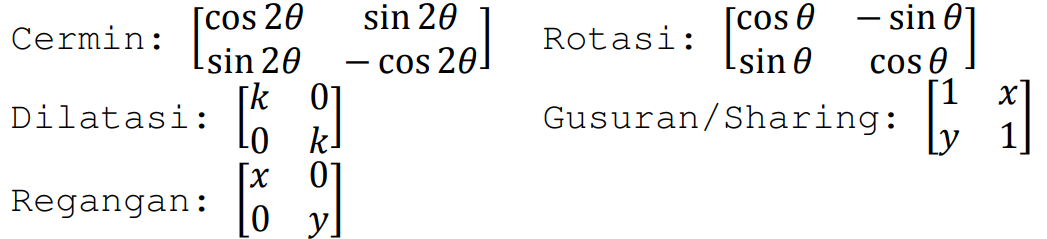
\includegraphics[width=\linewidth]{source/5-maths/Temporary/Geometry-matrixTransform.png}

\subsection{Trigonometric Equations}
\begin{verbatim}
sin(3A)        = 3 sin(A) - 4 sin^3(A)
sin(A/2)       = ((1 – Cos A)/2)^0.5
2 sin(A) cos B = sin(A+B) + sin(A-B)
tan(A) + tan(B) + tan(C) = tan(A) tan(B) tan(C); A+B+C= PI
\end{verbatim}

\begin{multicols}{2}
\textbf{Lingkaran Singung Segitiga}
\begin{verbatim}
a: (s(s-b)(s-c)/(s-a))^0.5
b: (s(s-a)(s-c)/(s-b))^0.5
c: (s(s-a)(s-b)/(s-c))^0.5
\end{verbatim}
\vfill\null\columnbreak
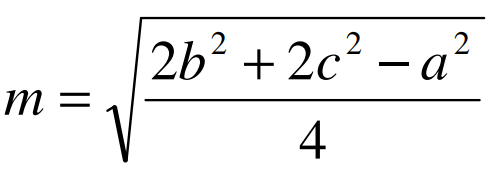
\includegraphics[width=0.6\linewidth]{source/5-maths/Temporary/Geometry-lingkaranSinggungSegitiga.png}
\end{multicols}

\textbf{Titik ke Garis}
\begin{verbatim}
U = ((x3-x1)(x2-x1)+(y3-y1)(y2-y1))/((x2-x1)^2+(y2-y1)^2)
X = x1 + U(x2-x1)
Y = y1 + U(y2-y1)
\end{verbatim}

\begin{multicols}{2}
\textbf{Dalil Steward} \\
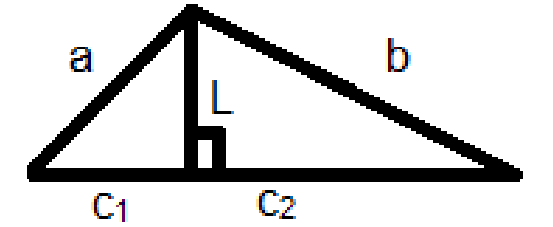
\includegraphics[width=0.5\linewidth]{source/5-maths/Temporary/Geometry-dalilSteward.png} \\
$L^2 . c = a^2.c_2 + b^2.c_1 - c_1.c_2.c$
\vfill\null\columnbreak
\textbf{Dalil Proyeksi} \\
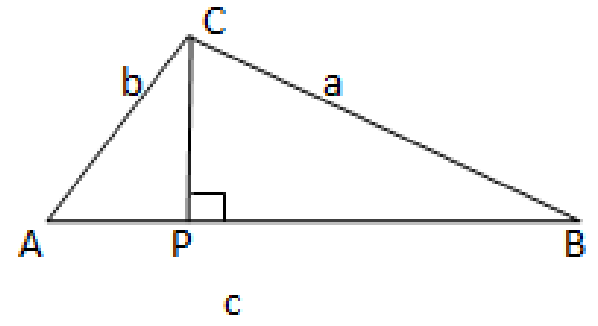
\includegraphics[width=0.5\linewidth]{source/5-maths/Temporary/Geometry-dalilProyeksi.png} \\
$AP = ( b^2 + c^2 - a^2 ) / 2c$
\end{multicols}

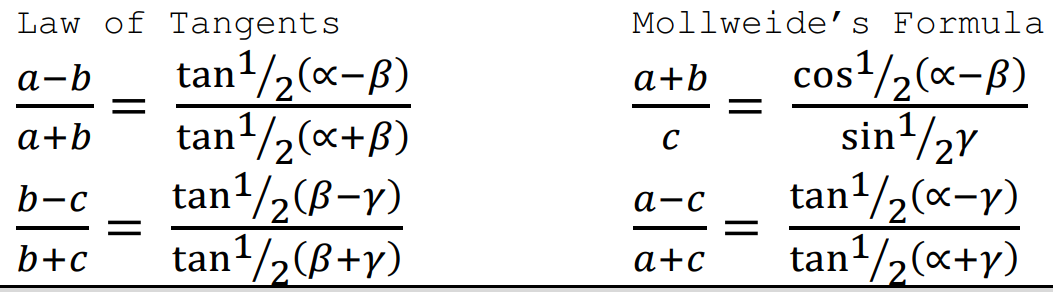
\includegraphics[width=0.8\linewidth]{source/5-maths/Temporary/Geometry-lawOfTangents.png}


% ====================================================================================================
% Geometry
\section{Geometry}
\lstset{inputpath=source/7-geometry/}

\subsection{Polygon Centroid and Area}
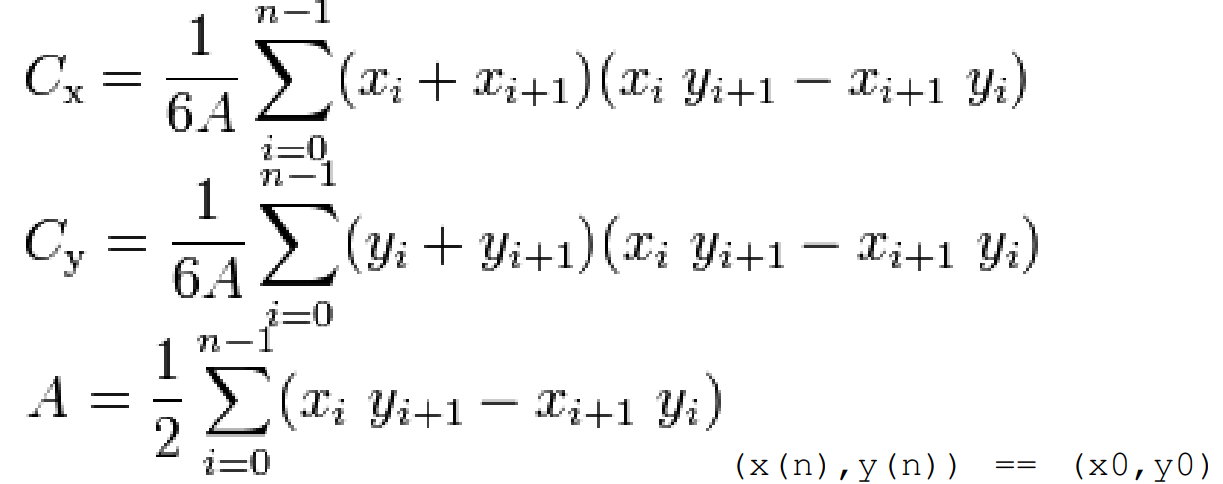
\includegraphics[width=\linewidth]{source/7-geometry/Temporary/Polygon-centroidAndArea.png}

\subsection{Line Segment Intersection Point}
\begin{huge}
  $\displaystyle D = (x_1 - x_2)(y_3 - y_4) - (y_1 - y_2)(x_3 - x_4)$ \\
  \\
  $\displaystyle x = \tfrac{1}{D} ((x_1y_2 - y_1x_2)(x_3 - x_4) - (x_3y_4 - y_3x_4)(x_1 - x_2))$ \\
  \\
  $\displaystyle y = \tfrac{1}{D} ((x_1y_2 - y_1x_2)(y_3 - y_4) - (x_3y_4 - y_3x_4)(y_1 - y_2))$
\end{huge}


\subsection{Line Segment Intersection}
\lstinputlisting[language=c++]{LineSegment-intersection.cpp}

\subsection{Square Collision}
\begin{verbatim}
((x1>=x1t && x1<=x2t) &&
 ((y1>=y1t && y1<=y2t) || (y2>=y1t && y2<=y2t) || (y1<=y1t && y2>=y2t))) ||
((x2>=x1t && x2<=x2t) &&
 ((y1>=y1t && y1<=y2t) || (y2>=y1t && y2<=y2t) || (y1<=y1t && y2>=y2t))) ||
((x1<=x1t && x2>=x2t) &&
 ((y1>=y1t && y1<=y2t) || (y2>=y1t && y2<=y2t) || (y1<=y1t && y2>=y2t)))
\end{verbatim}


\subsection{Closest Pair}
\lstinputlisting[language=c++]{ClosestPair.cpp}

\subsection{Polygon Class}
\lstinputlisting[language=c++]{Polygon-class.cpp}

\subsection{Point to Line}
\lstinputlisting[language=c++]{Point-toLine.cpp}

\subsection{Line to Segment}
\lstinputlisting[language=c++]{Line-toSegment.cpp}

\subsection{Polygon Diameter}
\lstinputlisting[language=c++]{Polygon-diameter.cpp}

\subsection{Union Rectangle Intersection}
\lstinputlisting[language=c++]{Rectangle-unionIntersection.cpp}

\subsection{Great Circle Distance}
\lstinputlisting[language=c++]{Sphere-GreatCircleDistance.cpp}